\documentclass[11pt, oneside]{article}   	% use "amsart" instead of "article" for AMSLaTeX format
\usepackage{geometry}                		% See geometry.pdf to learn the layout options. There are lots.
\geometry{letterpaper}                   		% ... or a4paper or a5paper or ... 
%\geometry{landscape}                		% Activate for for rotated page geometry
%\usepackage[parfill]{parskip}    		% Activate to begin paragraphs with an empty line rather than an indent
\usepackage{graphicx}				% Use pdf, png, jpg, or eps� with pdflatex; use eps in DVI mode
								% TeX will automatically convert eps --> pdf in pdflatex		
\usepackage{amssymb}
\usepackage{listings}

\title{CS 325: Project 1}
\author{Group 29: Jacob Mastel, Yash Naik, Cera Olson}
\date{}							% Activate to display a given date or no date

\begin{document}
\maketitle
\section{Algorithm 1: Enumeration}
\subsection{Theoretical Run-Time Analysis}

Enumeration has a running time of $O(n^{3})$. Because of the 3 loops, each run n times gives the algorithm a running time of ${n*n*n}$.

\subsection{Experimental Analysis}
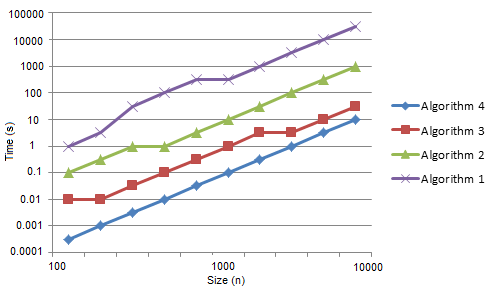
\includegraphics{AvgRunTime.png} \\
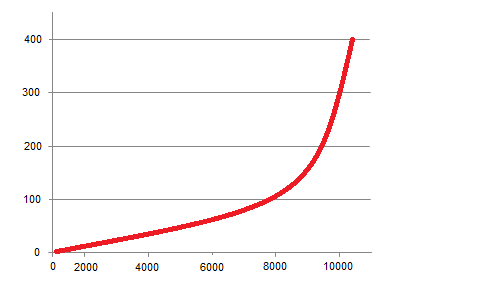
\includegraphics{Alg1Log.png}


\subsection{Extrapolation and Interpretation}

\subsubsection{For each algorithm use the experimental data to estimate a function that models the relationship between running times and input sizes (n). Discuss any discrepancies between the experimental and theoretical running times.}

\subsubsection{For each algorithm, what is the size of the biggest instance that you can solve with your algorithm in one hour?}

\section{Algorithm 2: Better Enumeration}
\subsection{Theoretical Run-Time Analysis}

\subsection{Experimental Analysis}
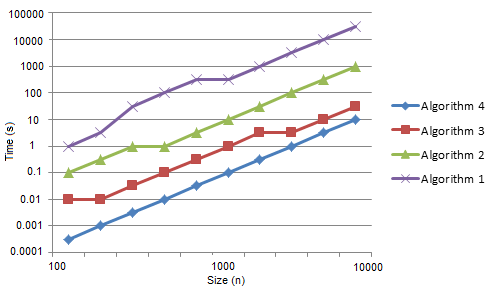
\includegraphics{AvgRunTime.png} \\
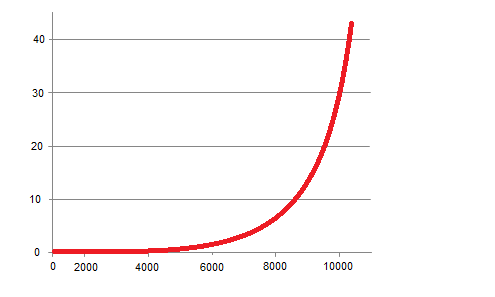
\includegraphics{Alg2Log.png}


\subsection{Extrapolation and Interpretation}
\subsubsection{For each algorithm use the experimental data to estimate a function that models the relationship between running times and input sizes (n). Discuss any discrepancies between the experimental and theoretical running times.}

\subsubsection{For each algorithm, what is the size of the biggest instance that you can solve with your algorithm in one hour?}

\section{Algorithm 3: Divide and Conquer}

\subsection{Theoretical Run-Time Analysis}

\subsection{Proof of Correctness}

\subsection{Experimental Analysis}
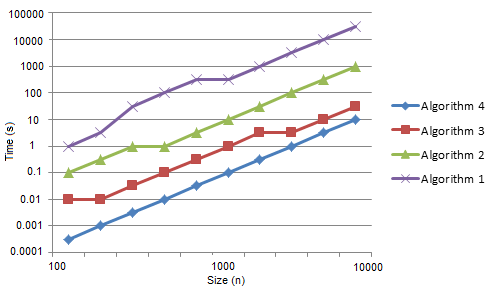
\includegraphics{AvgRunTime.png} \\
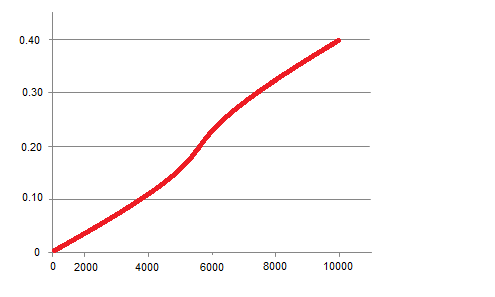
\includegraphics{Alg3Log.png}


\subsection{Extrapolation and Interpretation}
\subsubsection{For each algorithm use the experimental data to estimate a function that models the relationship between running times and input sizes (n). Discuss any discrepancies between the experimental and theoretical running times.}

\subsubsection{For each algorithm, what is the size of the biggest instance that you can solve with your algorithm in one hour?}

\section{Algorithm 4: Linear-Time}
\subsection{Theoretical Run-Time Analysis}

\subsection{Experimental Analysis}
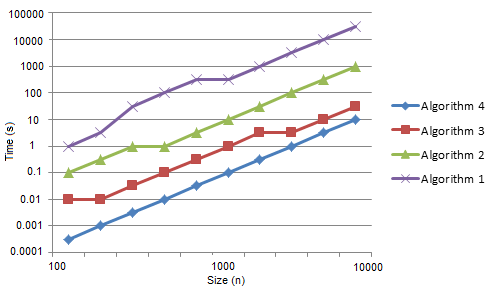
\includegraphics{AvgRunTime.png} \\
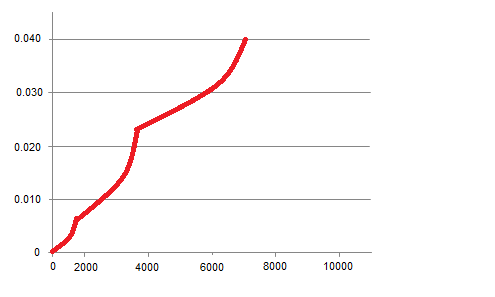
\includegraphics{Alg4Log.png}


\subsection{Extrapolation and Interpretation}
\subsubsection{For each algorithm use the experimental data to estimate a function that models the relationship between running times and input sizes (n). Discuss any discrepancies between the experimental and theoretical running times.}

\subsubsection{For each algorithm, what is the size of the biggest instance that you can solve with your algorithm in one hour?}

\newpage{}
\section{Appendices}
\subsection{Code}
\subsubsection{Algorithm 1}
\begin{verbatim}
def algorithm1(A):
	max = 0
	for i in range(0, len(A)):
		for j in range(i, len(A)):
			partial = 0
			for k in range(i, j+1):
				partial += A[k]

			if partial > max:
				max = partial

	return max
\end{verbatim}	
\subsubsection{Algorithm 2}
\begin{verbatim}
def algorithm2(A):
	max = 0
	for i in range(0, len(A)):
		sum = 0
		for j in range(i, len(A)):
			sum = sum + A[j]
			if max <= sum:
				max = sum

	return max
\end{verbatim}	
\subsubsection{Algorithm 3}
\begin{verbatim}
def algorithm3(A):
	if len(A) < 1:
		return 0

	m = len(A) / 2

	lmax = s = 0
	for i in range(len(A)/2, -1, -1):
		s += A[i]
		if s > lmax:
			lmax = s

	rmax = s = 0
	for i in range(len(A)/2+1, len(A)):
		s += A[i]
		if s > rmax:
			rmax = s

	return max(
		algorithm3(A[:len(A)/2]),
		algorithm3(A[(len(A)/2)+1:]),
		lmax + rmax
	)
\end{verbatim}	
\subsubsection{Algorithm 4}
\begin{verbatim}
def algorithm4(A):
	m1 = m2 = 0

	for x in A:
		m1 = max(0, m1 + x)
		m2 = max(m2, m1)

	return m2
\end{verbatim}	

\subsection{Tests}
\begin{verbatim}
# Algorithm Tests

# Needed Python libraries
import csv
import sys
import random
from timeit import Timer
from multiprocessing import Process

# Import our algorithms
from algorithm1 import *
from algorithm2 import *
from algorithm3 import *
from algorithm4 import *

# Global Variables
max_time = 2*60 # 2 minutes
min_num = -99
max_num = 99

def run_test(Alg):
	f_name = "alg_res{0}.csv".format(Alg)
	with open(f_name, 'wb') as csvfile:
		writer = csv.writer(csvfile)

		for n in range(100, 100001, 100):
			# build a random array of len n
			A = []
			for _ in range(n):
				A.append(random.randint(min_num, max_num))

			# determine which algorithm to call
			# run each set 3 times
			if Alg == 1:
				t = Timer(lambda: algorithm1(A)).timeit(number=3)
			elif Alg == 2:
				t = Timer(lambda: algorithm2(A)).timeit(number=3)
			elif Alg == 3:
				t = Timer(lambda: algorithm3(A)).timeit(number=3)
			elif Alg == 4:
				t = Timer(lambda: algorithm4(A)).timeit(number=3)

			writer.writerow([n, t])

			# see if we've gone beyond our max time.
			# if we have, break the loop
			if t >= max_time:
				break;

		print 'Algorithm {0} finished'.format(Alg)

def random_tests():
	jobs = []
	for i in range(1,5):
		p = Process(target=run_test, args=(i,))
		jobs.append(p)
		p.start()

	for p in jobs:
		p.join()

def print_fail(alg, a, expected, returned):
	print "Algorithm {0} failed test {1}".format(alg, a)
	print "  Expected: {0}".format(expected)
	print "  Returned: {0}".format(returned)

# Test each of the algorithms against known arrays and their answers
def validate_algorithms():
	a = {}
	a["a1"] = [1, 4, -9, 8, 1, 3, 3, 1, -1, -4, -6, 2, 8, 19, -10, -11]
	a["a1_sub"] = [8, 1, 3, 3, 1, -1, -4, -6, 2, 8, 19]
	a["a1_ans"] = 34

	a["a2"] = [2, 9, 8, 6, 5, -11, 9, -11, 7, 5, -1, -8, -3, 7 -2]
	a["a2_sub"] = [2, 9, 8, 6, 5]
	a["a2_ans"] = 30

	a["a3"] = [10, -11, -1, -9, 33, -45, 23, 24, -1, -7 -8, 19]
	a["a3_sub"] = [23, 24, -1, -7, -8, 19]
	a["a3_ans"] = 50

	a["a4"] = [31,-41, 59, 26, -53, 58, 97, -93, -23, 84]
	a["a4_sub"] = [59, 26, -53, 58, 97]
	a["a4_ans"] = 187

	a["a5"] = [3, 2, 1, 1, -8, 1, 1, 2, 3]
	a["a5_sub"] = [3, 2, 1, 1]
	a["a5_ans"] = 7

	a["a6"] = [12, 99, 99, -99, -27, 0, 0, 0, -3,10]
	a["a6_sub"] = [12, 99, 99]
	a["a6_ans"] = 210

	a["a7"] = [-2, 1, -3, 4, -1, 2, 1, -5, 4]
	a["a7_sub"] = [4, -1, 2, 1]
	a["a7_ans"] = 6

	a["a8"] = [-1, -3 -5]
	a["a8_sub"] = []
	a["a8_ans"] = 0

	all_passed = True
	for i in range(1,9):
		a1 = algorithm1(a["a{0}".format(i)])
		a2 = algorithm2(a["a{0}".format(i)])
		a3 = algorithm3(a["a{0}".format(i)])
		a4 = algorithm4(a["a{0}".format(i)])

		if  a1 != a["a{0}_ans".format(i)]:
			print_fail(1, i, a["a{0}_ans".format(i)], a1)
			all_passed = False

		if  a2 != a["a{0}_ans".format(i)]:
			print_fail(2, i, a["a{0}_ans".format(i)], a2)
			all_passed = False

		if  a3 != a["a{0}_ans".format(i)]:
			print_fail(3, i, a["a{0}_ans".format(i)], a3)
			all_passed = False

		if  a4 != a["a{0}_ans".format(i)]:
			print_fail(4, i, a["a{0}_ans".format(i)], a4)
			all_passed = False

	if all_passed == True:
		print 'All tests passed! :)'

def MSS_test():
	print "MSS_Test stuff goes here"

def print_help():
	print "Program argument error!"
	print "  Valid arguments include time_test, alg_test, or MSS_test"

if __name__ == "__main__":
	if len(sys.argv) < 2 :
		print_help()
		sys.exit()

	if sys.argv[1] == "time_test":
		random_tests()
	elif sys.argv[1] == "alg_test":
		validate_algorithms()
	elif sys.argv[1] == "MSS_test":
		MSS_test()
	else:
		print_help()
\end{verbatim}		

\end{document}  